\usetikzlibrary{arrows.meta}
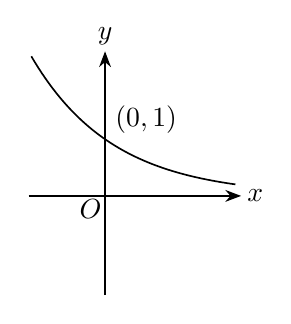
\begin{tikzpicture}[x=0.72cm,y=0.72cm,line width=.6pt,>=Stealth,font=\normalsize]
\draw[->] (-1.35,0)--(2.40,0) node[right,inner sep=0pt,xshift=2pt] {$x$};
\draw[->] (0,-1.75)--(0,2.55) node[above,inner sep=0pt,yshift=2pt] {$y$};
\node[below left,inner sep=1pt] at (0,0) {$O$};
\draw[domain=-1.30:2.30,samples=180] plot (\x,{2^(-\x)});
\node[anchor=south west,inner sep=1pt] at (0.12,1.04) {$(0,1)$};
\end{tikzpicture}
